\documentclass[a4paper,german,12pt,smallheadings]{scrartcl}
\usepackage[T1]{fontenc}
\usepackage[utf8]{inputenc}
\usepackage{babel}
\usepackage{geometry}
\usepackage[fleqn]{amsmath}
\usepackage{amssymb}
\usepackage{float}
\usepackage{enumerate}
\usepackage{commath} % http://tex.stackexchange.com/questions/14821/whats-the-proper-way-to-typeset-a-differential-operator
\usepackage{cancel}
\usepackage{pdfpages}

\usepackage[fleqn]{mathtools}
% Number only referenced equations
%\mathtoolsset{showonlyrefs}

%\usepackage{wrapfig}
\usepackage[thinspace,thinqspace,squaren,textstyle]{SIunits}
\usepackage{tikz}
\usepackage[europeanresistors]{circuitikz}

% New command for color underlining
\usepackage{xcolor}

\newsavebox\MBox
\newcommand\colul[2][red]{{\sbox\MBox{$#2$}%
  \rlap{\usebox\MBox}\color{#1}\rule[-1.2\dp\MBox]{\wd\MBox}{0.5pt}}}

\restylefloat{table}
\geometry{a4paper, top=15mm, left=20mm, right=10mm, bottom=20mm, headsep=10mm, footskip=12mm}
\linespread{1.5}
\setlength\parindent{0pt}
\DeclareMathOperator{\Tr}{Tr}
\DeclareMathOperator{\Var}{Var}
\begin{document}
\allowdisplaybreaks % Seitenumbrüche in Formeln erlauben
\begin{center}
\bfseries % Fettdruck einschalten
\sffamily % Serifenlose Schrift
\vspace{-40pt}
Physikalisches Grundpraktikum 2, Wintersemester 2014/2015

Markus Fenske \texttt{<iblue@zedat.fu-berlin.de>}

Diode, Tutor: Andreas Maier
\vspace{-10pt}
\end{center}
\section{Einführung}
Ziel des Versuches ist die Aufnahme der Strom/Spannungs-Kennlinie einer
Halbleiterdiode und der Aufbau einer Gleichrichterschaltung (Gratzschaltung).

\section{Theoretische Grundlagen}

\subsection{Halbleiterdiode}

Die Diode ist ein Bauelement, das einen Stromfluss nur in eine Richtung (die
Durchlassrichtung) zulässt. Wir die Diode in Sperrrichtung betrieben, findet
kein Stromfluss statt.

\subsubsection{Aufbau}

Halbleiterkristalle können dotiert werden. Dazu werden in den
Halbleiterkristall Fremdatome eingebracht die zu Störstellen im Kristall führen
und somit seine Eigenschaften ändern. Man unterscheidet dabei zwischen
negativer und positiver Dotierung (n- und p-Dotierung).

\begin{figure}[H]
  \centering
  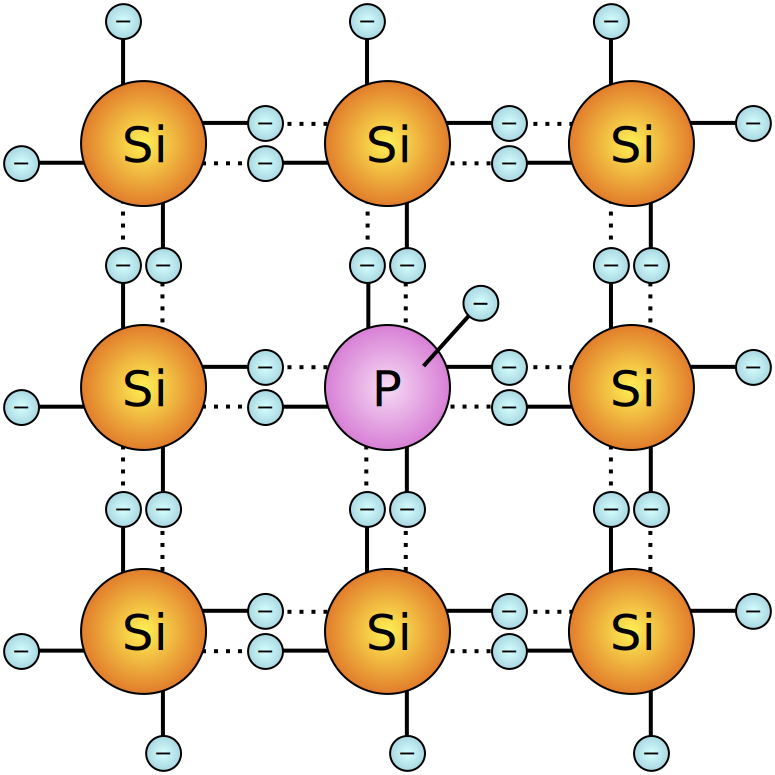
\includegraphics[width=.3\textwidth]{ndot.pdf}
  \label{img:ndot}
  \caption{n-Dotierung: Einbringen eines Fremdatoms zur Erzeugung eines Elektronenüberschusses}
\end{figure}

Als Beispiel der n-Dotierung wird in einen Silizium-Kristall (der über 4
Valenzelektronen verfügt) ein Phosphor-Atom eingebaut (das über 5
Valenzelektronen verfügt). Somit befindet sich im Kristall ein
Elektronenüberschuss (siehe Abbildung \ref{img:ndot}).

\begin{figure}[H]
  \centering
  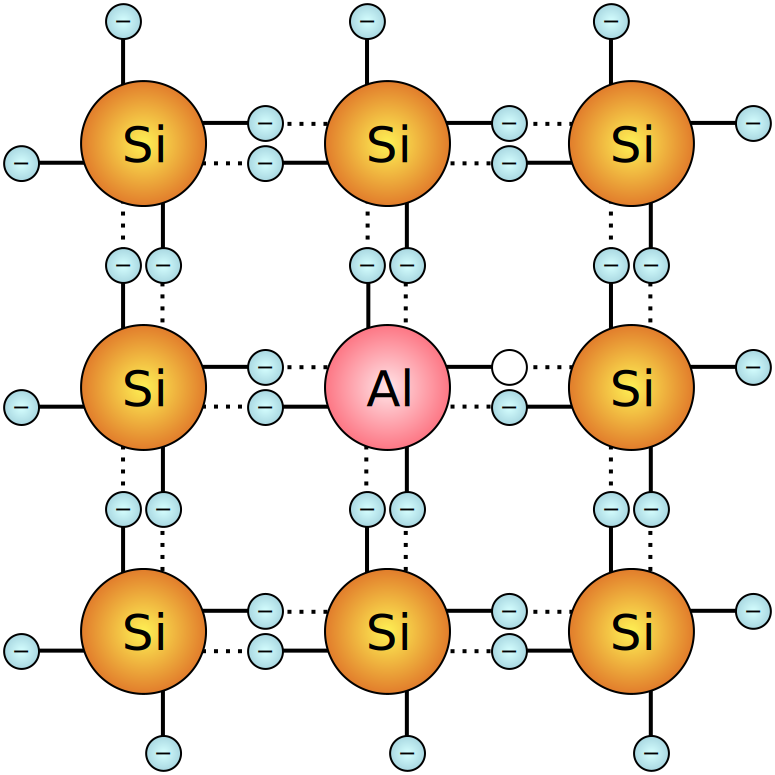
\includegraphics[width=.3\textwidth]{pdot.pdf}
  \label{img:pdot}
  \caption{p-Dotierung: Einbringen eines Fremdatoms zur Erzeugung einer Fehlstelle}
\end{figure}

Bei der p-Dotierung wird hingegen ein Aluminium-Atom (das über 3
Valenzelektronen) verfügt in den Kristall eingefügt. Es entsteht eine
Fehlstelle im Kristall (sog. Loch) (siehe Abbildung \ref{img:pdot}).

\begin{figure}[H]
  \centering
  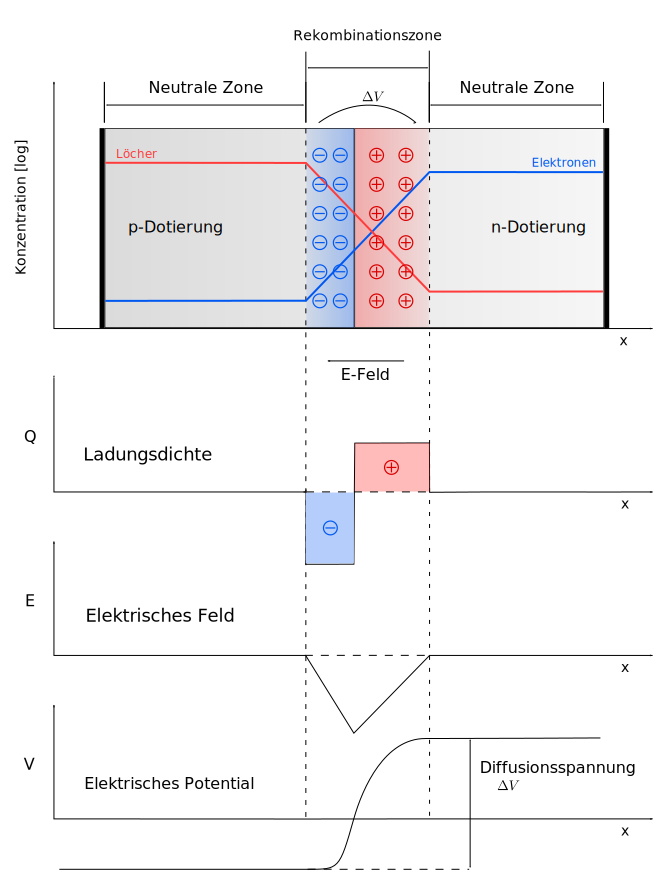
\includegraphics[width=.6\textwidth]{pnjunct.pdf}
  \label{img:pnjunct}
  \caption{p-n-Übergang}
\end{figure}

Eine Diode besteht nun aus einem p-n-Übergang. Das bedeutet, die beiden
dotierten Kristalle werden in direkten Kontakt miteinander gebracht. Dabei
rekombinieren die Elektronen mit den Löchern. Es entsteht ein elektrisches
Potential, das eine Sperrschicht bildet (siehe Abbildung
\ref{img:pnjunct}).

\subsubsection{Betrieb in Sperrrichtung}

Wird an die Diode eine Spannung angelegt (Minus am n-Kristall, Plus am
p-Kristall), kommen die Elektronen vom Minuspol und Rekombinieren mit den
Löchern. Dabei wird die Raumladungszone verbreitert und damit das zu
überwindende Potential höher. Es kann kein Strom fließen.

Wird irgendwann das Potential so groß, dass die Rekombinationszone gesättigt
wird und ist das Potential hoch genug, kommt es dennoch zum Durchtunneln
einzelner Elektronen (sog. Durchbruch). Diesen werden wir aber nicht messen.

\subsubsection{Betrieb in Durchlassrichtung}

Wird die Spannung anders herrum angelegt (Minus am p-Kristall, Plus am
n-Kristall) führt das dazu, dass die Elektronen die positive Ladung auf der
n-Seite kompensieren. Die Elektronen auf der p-Seite werden vom anliegenden
Potential zum Abfließen bewegt, somit verkleinert sich die Raumladungszone. Ist
die angelegte Spannung hoch genug (Durchlassspannung), ist die Raumladungszone
so klein, dass einzelne Elektronen durchtunneln können. Es beginnt ein Strom zu
fließen. Je hoher das Potential wird, desto kleiner wird die Raumladungszone
und desto mehr Elektronen fließen.

\subsubsection{Shockley-Gleichung}

Der Zusammenhang zwischen Strom- und Spannung an einer Diode wird durch die
Schockley-Gleichung angegeben. Diese lässt sich nur durch statistische
Betrachtungen an Halbleiterkristallen herleiten, weswegen ich auf die
Herleitung nicht genauer eingehen werde. Sie lautet:

\begin{equation}
  I_D = I_S \del{e^{U_D}{n U_T} - 1}
\end{equation}

Dabei gibt $I_D$ den Stromfluss durch die Diode bei einer angelegten Spannung
$U_D$ an. $n$ ist der materialabhängige Emissionskoeffizient ($n \in [1,2]$).
$U_T$ ist die Temperaturspannung $U_T = k_B T/q$ (mit $k_B$:
Boltzmann-Konstante, $T$: Temperatur, $q$: Elementarladung). Sie beträgt bei
Raumtemperatur etwa $25 \;\operatorname[mV]$.

\begin{figure}[H]
  \centering
  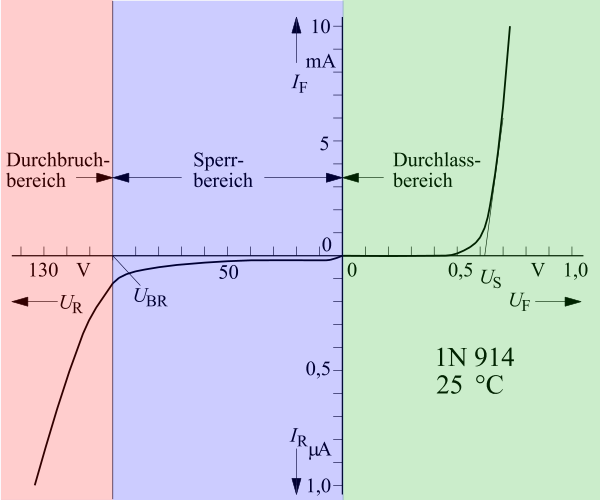
\includegraphics[width=.6\textwidth]{kennlinie.pdf}
  \label{img:kennlinie}
  \caption{Kennlinie einer Diode}
\end{figure}

Der Verlauf in Sperrrichtung folgt hingegen anderen Zusammenhängen, auf die
wir nicht weiter eingehen wollen, da wir diese nicht messen. Der Verlauf der
gesamten Kennlinie wird in Abbildung \ref{img:kennlinie} wiedergegeben.


\subsection{Elektrotechnische Betrachtungen}

\begin{figure}[H]
  \begin{center}
    \begin{circuitikz}
      \draw (0,0) to[Do] (2,0);
    \end{circuitikz}
    \caption{Schaltzeichen der Diode}
    \label{img:diode}
  \end{center}
\end{figure}

Das Schaltzeichen für die Diode ist in Abbilung \ref{img:diode} aufgeführt. Der
Pfeil zeigt dabei die Durchlassrichtung an, dabei gilt technische Stromrichtung
(also Stromfluss von Plus nach Minus).

\subsubsection{Einfacher Gleichrichter}

\begin{figure}[H]
  \begin{center}
\begin{tikzpicture}
    \draw (6,4) node[ocirc,label={right:+}] {};
    \draw (6,0) node[ocirc,label={right:--}] {};
    \draw (6,0)
      to[short] (0,0)
      to[sV] (0,4)
      to[Do] (6,4);

\end{tikzpicture}
    \caption{Einfacher Gleichrichter}
    \label{img:graetz}
  \end{center}
\end{figure}

\begin{figure}[H]
  \begin{center}
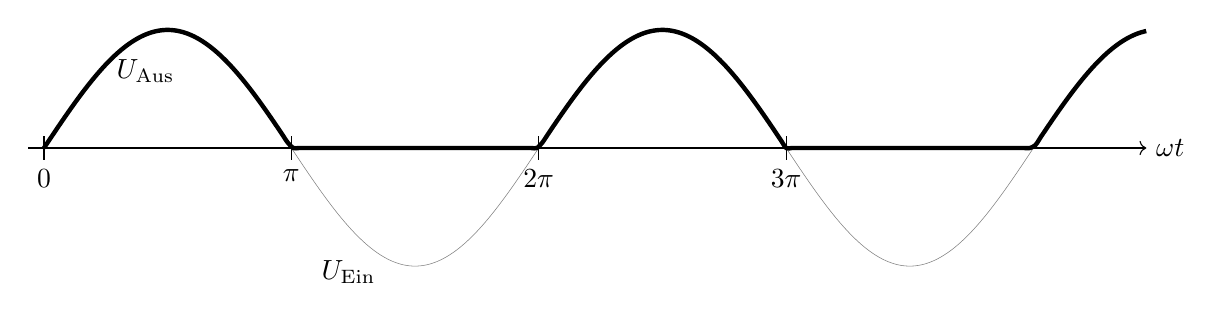
\begin{tikzpicture}
\begin{scope}[xscale=1,yscale=1.5]
    \draw[thin, ->] (-0.2, 0) -- (14,0) node[right] {$\omega t$};

    \foreach \x/\xtext in {0,{pi}/\pi,{2*pi}/{2\pi},{3*pi}/{3\pi}}
        \draw (\x,0.1) -- (\x,-0.1) node [below] {$\xtext$};


    % Vs
    \draw[domain=0:14, samples=200, help lines, smooth]
        plot (\x,{sin(\x r)});
    % U_0
    \draw[domain=0:14, samples=200, ultra thick, smooth]
      plot (\x,{max(sin(\x r), 0)});
    % U_Glatt
    %\draw[domain=0:14, thick, smooth]
    %  plot (\x,{1});
    \node[right] at (.8,.65) {$U_\text{Aus}$};
    %\node[right] at (1.7,1.25) {$U_\text{Glatt}$};
    \node[right] at ({pi+pi/12},-1.05) {$U_\text{Ein}$};
\end{scope}
\end{tikzpicture}
    \caption{Ein- und Ausgangsspannung des einfachen Gleichrichters}
    \label{img:simprectout}
  \end{center}
\end{figure}

Mithilfe der Diode lassen sich Wechselströme gleichrichten. Der naive Ansatz
ist dabei, eine einzelne Diode in Reihe zu einem Gleichstromverbraucher zu
schalten. Die Diode sperrt dann die negativen Halbwellen und lässt die
positiven durch. Dabei kann man jedoch nur jede zweite Halbwelle nutzen.

\subsubsection{Graetzschaltung}
\begin{figure}[H]
  \begin{center}
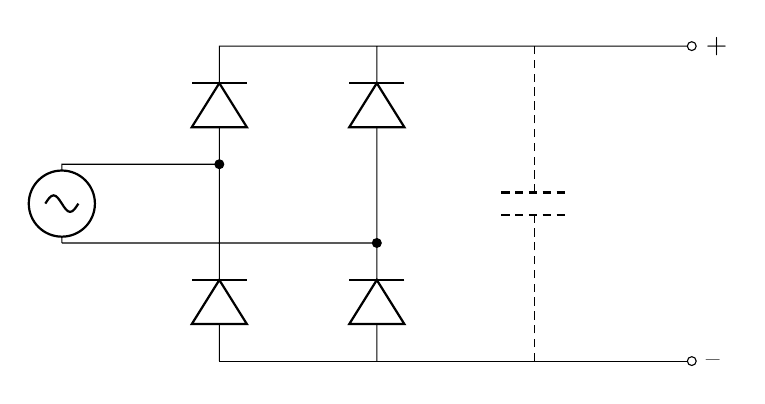
\begin{tikzpicture}
    \draw
    (2,0)
    % Diode leg 1
        to[Do] ++(0,1.5)
        -- ++(0,1)
        to[Do] ++(0,1.5) coordinate (leg2)
    % Diode leg 1
    (0,0)
        to[Do] ++(0,1.5)
        -- ++(0,1)
        to[Do] ++(0,1.5) coordinate (leg1)
    % Connections and load R
        -- ++(3,0)
        to[short] ++(3,0)
        %-- ++(0,-0.8)
        %to[R=$R_L$] ++(0,-2.4)
        %to[R] ++(0,-1.2)
        %to[L] ++(0,-1.2)
    % Back to (0,0)
        %|- (0,0)
    % AC source
    (-2,1.5) coordinate (Vnn)
        to[sV] ++(0,1) coordinate (Vpp)
        -- (leg1 |- Vpp) node [circ] {}
    (Vnn)
        -- (leg2 |- Vnn) node [circ] {}
    ;
    \draw (0,0) |- (6,0);
    \draw (6,4) node[ocirc,label={right:+}] {};
    \draw (6,0) node[ocirc,label={right:--}] {};
    \draw [densely dashed] (4,0) to[C] (4,4);
\end{tikzpicture}
    \caption{Graetzschaltung mit optionalem Glättungskondensator}
    \label{img:graetz}
  \end{center}
\end{figure}
\begin{figure}[H]
  \begin{center}
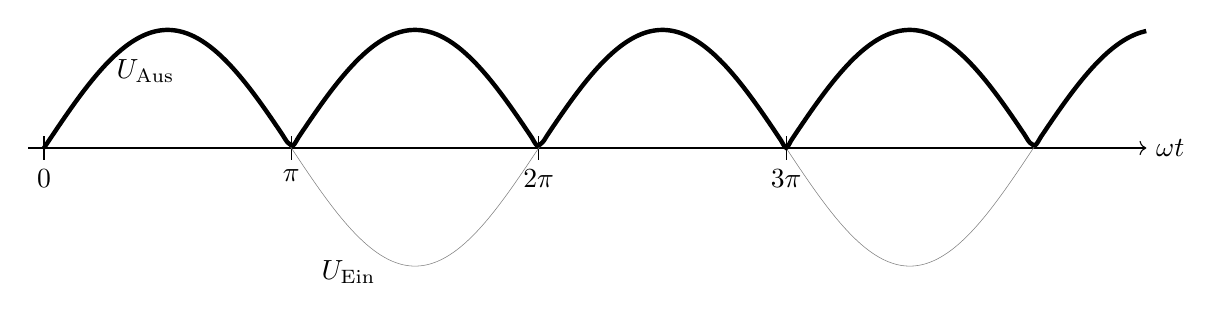
\begin{tikzpicture}
\begin{scope}[xscale=1,yscale=1.5]
    \draw[thin, ->] (-0.2, 0) -- (14,0) node[right] {$\omega t$};

    \foreach \x/\xtext in {0,{pi}/\pi,{2*pi}/{2\pi},{3*pi}/{3\pi}}
        \draw (\x,0.1) -- (\x,-0.1) node [below] {$\xtext$};


    % Vs
    \draw[domain=0:14, samples=200, help lines, smooth]
        plot (\x,{sin(\x r)});
    % U_0
    \draw[domain=0:14, samples=200, ultra thick, smooth]
      plot (\x,{abs(sin(\x r))});
    % U_Glatt
    %\draw[domain=0:14, thick, smooth]
    %  plot (\x,{1});
    \node[right] at (.8,.65) {$U_\text{Aus}$};
    %\node[right] at (1.7,1.25) {$U_\text{Glatt}$};
    \node[right] at ({pi+pi/12},-1.05) {$U_\text{Ein}$};
\end{scope}
\end{tikzpicture}
    \caption{Ein- und Ausgangsspannung einer Graetzschaltung}
    \label{img:graetzout}
  \end{center}
\end{figure}
Besser zur Gleichrichtung geeignet ist die Graetzschaltung. Dabei werden vier
Dioden genutzt (siehe Schaltung), um beide Halbwellen auszunutzen. Wir nehmen
dabei eine in erster Näherung lineare Kennlinie der Dioden an, um die
Betrachtung nicht zu komplex zu machen.


Wird noch ein Kondensator parallel zum Ausgang geschaltet, kann die Spannung
geglättet werden. Je nach Kennlinie der Dioden, angeschlossenem Verbraucher
usw. gibt es eine phasenverschobene Restwelligkeit. Die genaue Betrachtung ist
kompliziert und übersteigt die Aufgabenstellung. Da die intuitive Betrachtung
von nichtlinearen Wechselstromschaltkreisen zu falschen Ergebnissen führt,
sparen wir uns irgendwelche Mutmaßungen über das genaue Aussehen der
Ausgangsspannung in diesem Fall.



\end{document}
